\begin{figure}[ht]
  \centering
  \begin{subfigure}{0.14\linewidth}
 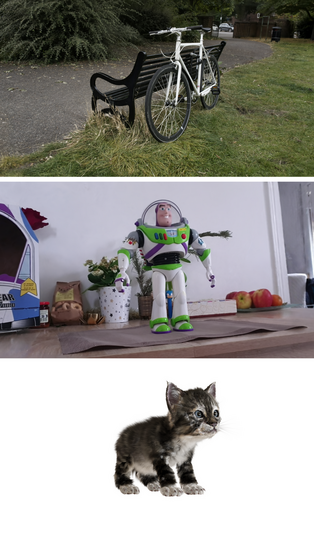
\includegraphics[width=\linewidth]{images/composition/buzz_riding_cat/scenes.png}
 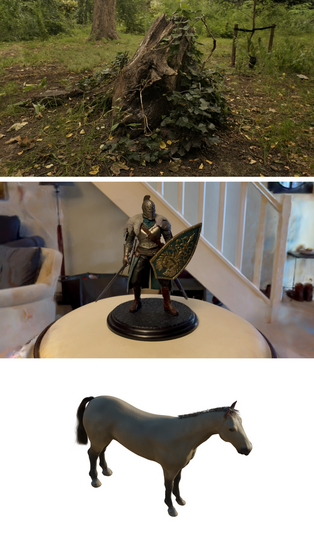
\includegraphics[width=\linewidth]{images/composition/knight_and_horse/scenes.png}
 \caption{Scenes}
  \end{subfigure}
  %
  \hfill
  %
  \begin{subfigure}{0.42\linewidth}
 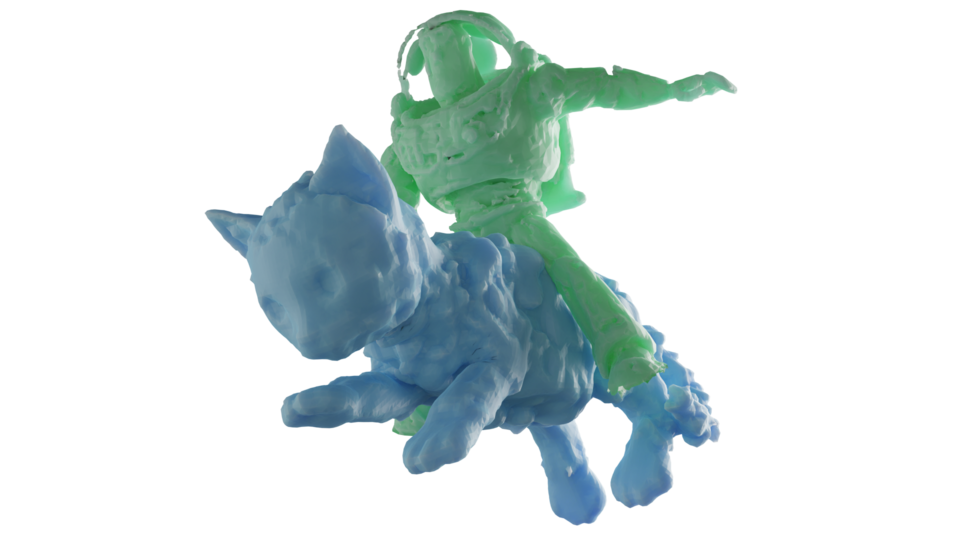
\includegraphics[width=\linewidth]{images/composition/buzz_riding_cat/mesh.png}
 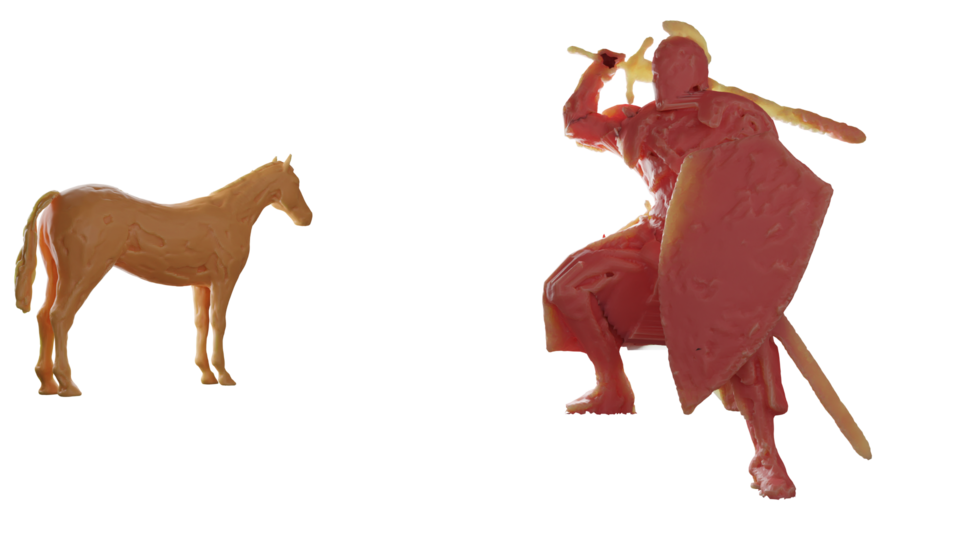
\includegraphics[width=\linewidth]{images/composition/knight_and_horse/mesh.png}
  \caption{Posing foreground meshes}
  \end{subfigure}
  %
  \hfill
  \begin{subfigure}{0.42\linewidth}
 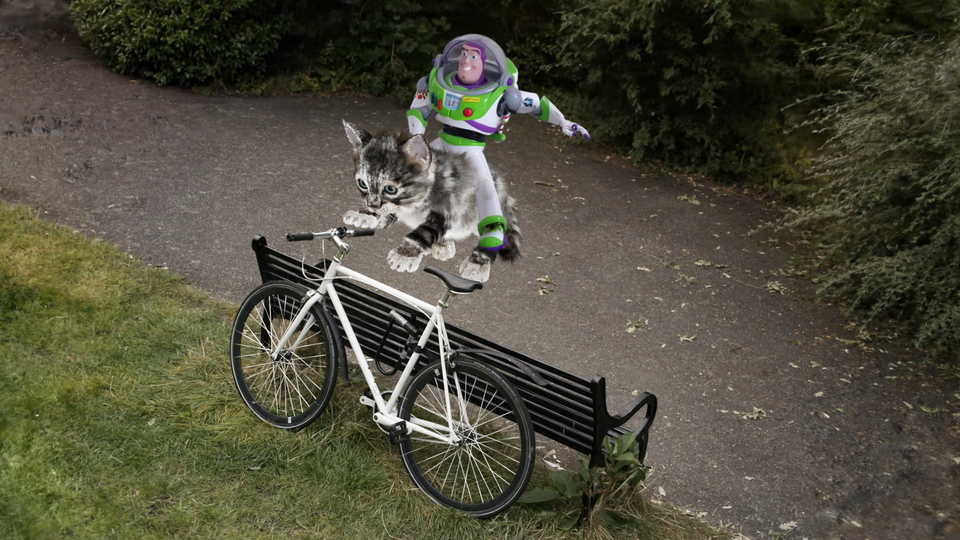
\includegraphics[width=\linewidth]{images/composition/buzz_riding_cat/0_0.png}
 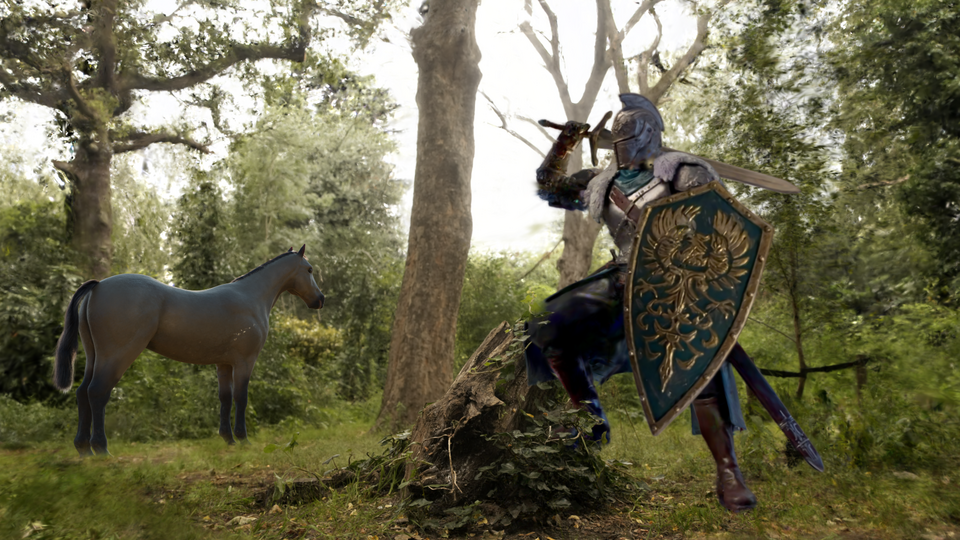
\includegraphics[width=\linewidth]{images/composition/knight_and_horse/0_1.png}
  \caption{Rendering composition}
  \end{subfigure}
  %
  \caption{
  \textbf{Scene composition.} Using mesh editing tools in Blender, we were able to combine various elements from multiple scenes (a) to build a whole new scene (c). We also changed the pose of the characters by using the rigging tool in Blender (b). Similarly to surface-based methods like SuGaR~\cite{guedon2023sugar}, Frosting can be used for editing and compositing scenes, but allows for better rendering of complex volumetric effects and fuzzy materials, such as hair or grass.
  }
  \label{fig:scene-composition}
\end{figure}